\documentclass[varwidth=true, border=2pt]{standalone}

\usepackage{tikz}
\usetikzlibrary{shapes,snakes,shapes.geometric,positioning}

\begin{document}
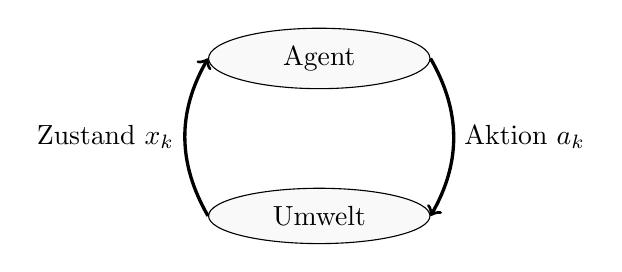
\begin{tikzpicture}[node distance=2cm]
    \node[ellipse,draw,minimum width=80pt,minimum height=20pt,fill=gray!5] (a) {Agent};
    \node[ellipse,draw,minimum width=80pt,minimum height=20pt,fill=gray!5,below of=a] (u) {Umwelt};

    % Arrows
    \draw[bend left,->,very thick] (a.east) to node [auto] {Aktion $a_k$} (u.east);
    \draw[bend left,->,very thick] (u.west) to node [auto] {Zustand $x_k$} (a.west);
\end{tikzpicture}
\end{document}
